%
% $RCSfile: common_knowledge_abstraction.tex,v $
%
% Copyright (C) 2002-2008. Christian Heller.
%
% Permission is granted to copy, distribute and/or modify this document
% under the terms of the GNU Free Documentation License, Version 1.1 or
% any later version published by the Free Software Foundation; with no
% Invariant Sections, with no Front-Cover Texts and with no Back-Cover
% Texts. A copy of the license is included in the section entitled
% "GNU Free Documentation License".
%
% http://www.cybop.net
% - Cybernetics Oriented Programming -
%
% http://www.resmedicinae.org
% - Information in Medicine -
%
% Version: $Revision: 1.1 $ $Date: 2008-08-19 20:41:05 $ $Author: christian $
% Authors: Christian Heller <christian.heller@tuxtax.de>
%

\subsection{Common Knowledge Abstraction}
\label{common_knowledge_abstraction_heading}
\index{Common Knowledge Abstraction}
\index{Software Engineering Process}
\index{SEP}
\index{Analysis}
\index{Design}
\index{Implementation}
\index{Abstraction Gaps}
\index{CYBOL}
\index{CYBOI}

Although this work does not address the \emph{Software Engineering Process}
(SEP) directly, its results have great effect on it, which this section wants to
shed some more light on. Classical SEP phases are: \emph{Analysis}, \emph{Design}
and \emph{Implementation} (chapter \ref{software_engineering_process_heading}).

\begin{figure}[ht]
    \begin{center}
        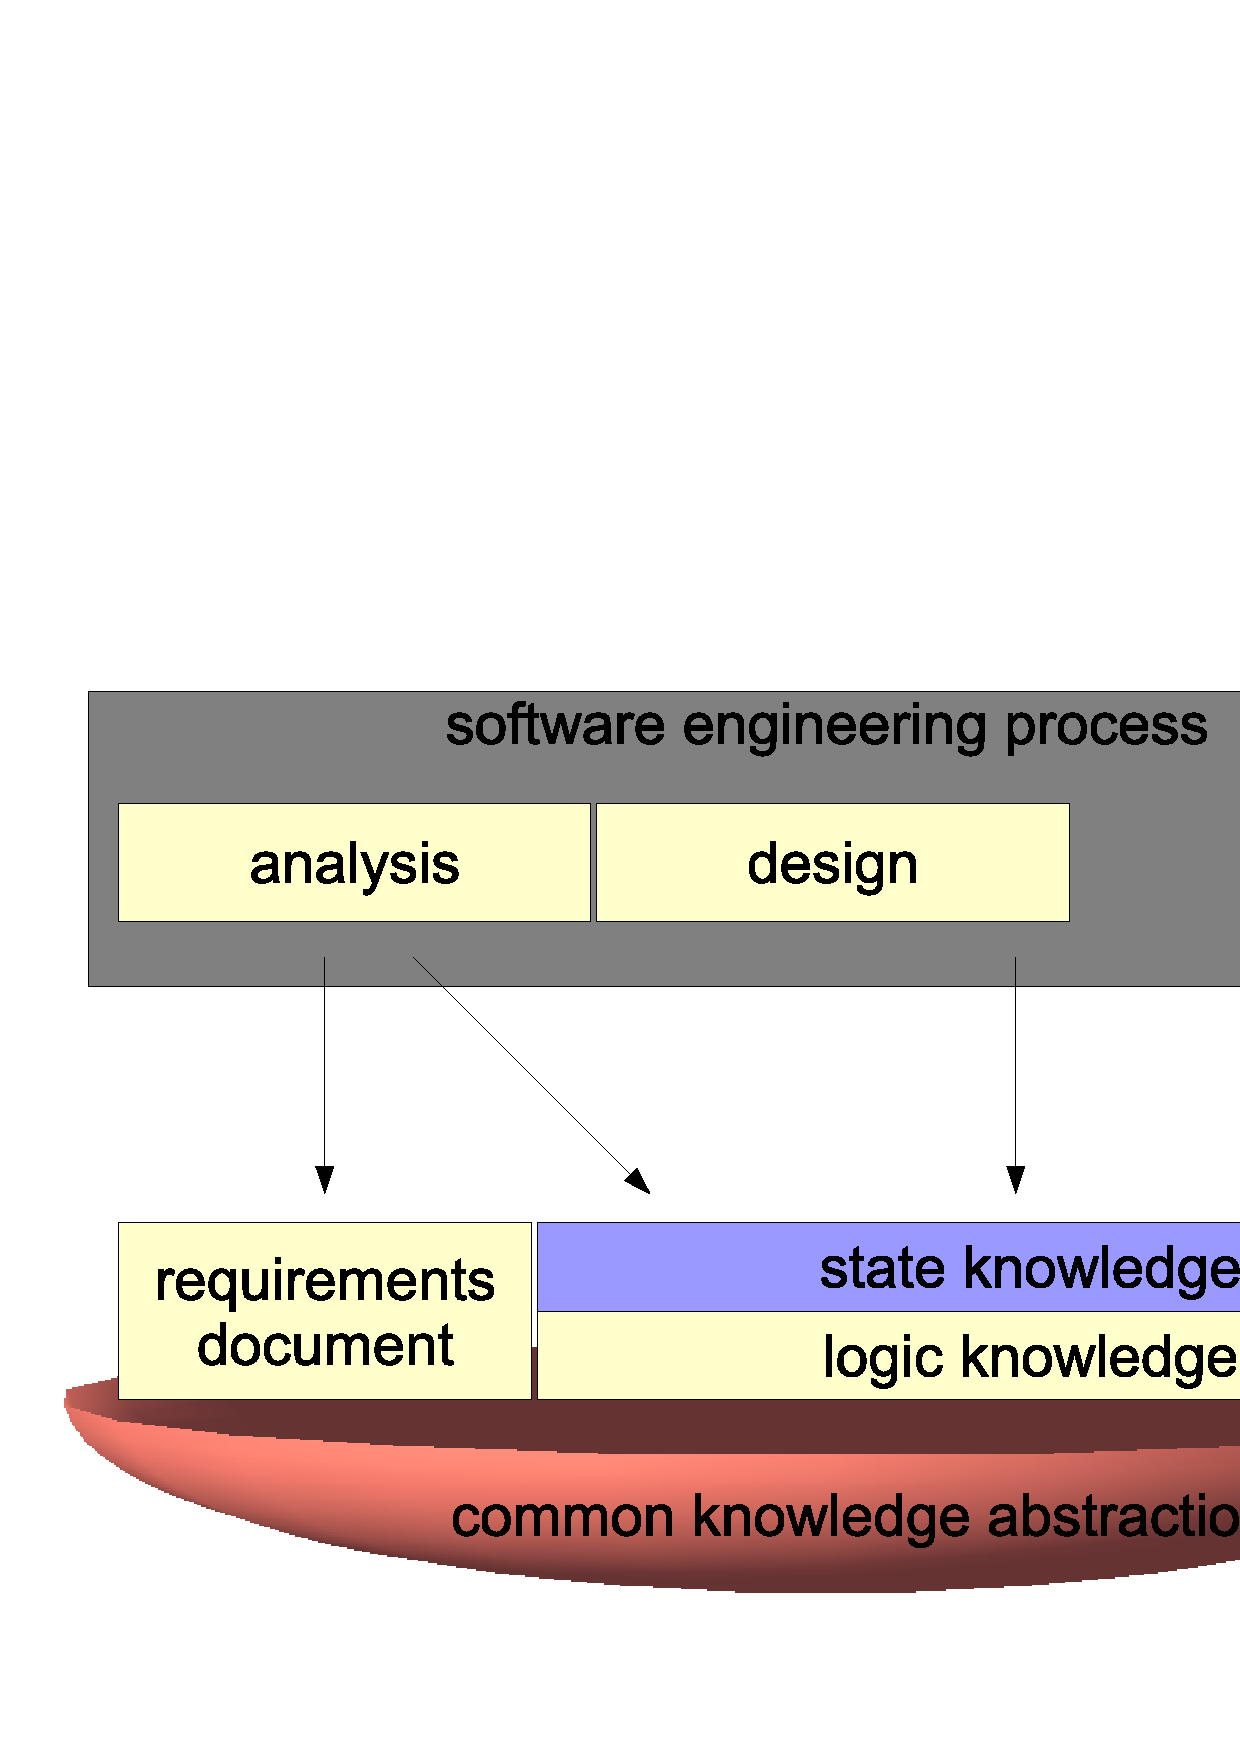
\includegraphics[scale=0.3,angle=-90]{graphic/common.pdf}
        \caption{Common Knowledge Abstraction useable by many SEP Phases}
        \label{common_figure}
    \end{center}
\end{figure}

Section \ref{abstraction_gaps_heading} pointed out abstraction gaps and
multiple development paradigm switches, happening during a software project's
lifetime. It set out to find a \emph{Common Knowledge Abstraction} for all
phases. The results of this work overcome \emph{Gap 2}, as shown in figure
\ref{gaps_figure}. Knowledge models as specified in this work can be used
throughout most project phases (figure \ref{common_figure}). Domain experts and
application developers work with platform-neutral knowledge templates. Since
these are interpreted, a translation into classical software source code is not
necessary anymore. CYBOL knowledge templates represent the designed
architecture \emph{and} implemented application, at the same time. The formerly
needed implementation phase thus disappears, which shortens the whole SEP. It
is hard to estimate the amount of saved time and costs.

Using CYBOL, experts can hopefully yet more actively contribute to application
development. Consequently, there may be less organisational problems in
projects and companies, if experts and system developers can independently
develop their parts (CYBOL vs. CYBOI) of the application system to be created.
The whole SEP may become more \emph{transparent} and \emph{understandable}, and
hopefully produce more \emph{flexible}, \emph{stable} and \emph{secure}
systems. However, the exact effort, especially to what concerns security issues
cannot be estimated yet and has to be investigated further.
